\section{Описание практической части}
\label{sec:Chapter4} \index{Chapter4}

% Если в рамках работы писался какой-то код, здесь должно быть его
% описание: выбранный язык и библиотеки и мотивы выбора, архитектура,
% схема функционирования, теоретическая сложность алгоритма, характеристики
% функционирования (скорость/память).

\subsection{Построение шаблона}
Для выполнения поставленных задач, прежде всего требуется оценить насколько часто конструкции, содержащие в себе ленивые вычисления, могут встречаться в коде. Для этого необходимо выбрать шаблон, по которому можно определить ленивые вычисления, требуемый для поиска потенциальных кандидатов для векторизации. Следует также определить стартовую точку для построения этого шаблона и реализовать отбор среди кандидатов на предмет наличия тех или иных зависимостей.

Определимся каким условиям должен удовлетворять шаблон, требуемый для задачи. 

\textit{Первым условием} является поиск стартовой точки, с которой будет начинаться построение шаблона. \textit{Стартовая точка} - определение начала участка кода, который будет подвергаться векторизации. В работе за стартовые точки векторизации были приняты операции чтения из памяти, поскольку в последующем они будут объединяться в одну операцию. Так как целью работы является векторизация ленивых вычислений, то все инструкции чтения из памяти не подходят. Необходимо найти такие инструкции обращения в память, которые находятся внутри условия if-else конструкции. Пример представлен на рисунке ~\ref{4lazy}.

\begin{figure}[!htb]
    \centering
    \includesvg[scale=1]{4lazy.svg}
    \caption{Пример шаблона ленивых вычислений, требуемый для поиска и векторизации}
    \label{4lazy}
\end{figure}

Соответственно, \textit{вторым условием} для построения шаблона является наличие инструкций ветвления. Поскольку оптимизация проводится на уровне IR, то непосредственный интерес представляют базовые блоки, конечными инструкциями которых являются условные переходы. Ввиду того, что для векторизации необходимо два или более обращений в память и каждое из условий if-else конструкции представлено отдельным базовым блоком из-за специфики самого IR и определения базового блока, то требуется найти цепочку из базовых блоков, связанных между собой условными переходами и удовлетворяющих условию выше.

Приступая к \textit{третьему условию}, необходимо напомнить, что базовые блоки соединены между собой дугами (подробнее в 1.2.2). Базовые блоки из набранной цепочки имеют две выходящих дуги, так как оканчиваются на условные переходы. Одна из дуг каждого базового блока должна быть входящей дугой для следующего, а вторая дуга должна соединять с одним и тем же базовым блоком, который по сути является продолжением потока управления в случае \textit{выполнения (оператор ИЛИ)} или же \textit{невыполнения (оператор И)} условия. Пример такого шаблона представлен на рис. ~\ref{bbchain}.

\begin{figure}[!htb]
    \centering
    \includesvg[scale=1]{bbchain.svg}
    \caption{Пример подходящей цепочки из базовых блоков для задачи}
    \label{bbchain}
\end{figure}

% Введем понятие шага векторизации.

% Шаг векторизации - это константа, равная размеру типа, или же в случае обращения по индексу массива, равная 1.
% \todo[убрать оставить только размер типа]

Самой сложной частью является определение \textit{соседства} операций чтения из памяти. Под \textit{соседством} в данном случае подразумевается, что данные в памяти лежат рядом друг с другом. В случае двух соседних элементов массива это гарантируется линейной моделью памяти, упоминаемой в пункте 3.3 в работе \cite{pohl2018control}. В коде же данное свойство представлено несколькими обращениями в память, отличающимися лишь смещением на константу, равную размеру типа. Например, на рисунке ~\ref{4lazy} все 4 операции обращения в память являются \textit{соседними}. 

Таким образом, \textit{четвертым условием} является поиск таких обращений в память, которые являются \textit{соседними}. Поскольку промежуточное представление использует SSA-форму (рассмотрено в главе 1.2.4), то задача поиска \textit{соседних} операций загрузки из памяти представляет собой задачу построения PSF-формы (подробнее в главе 1.2.6). В SSA-форме каждый объект имеет ровно одно \textit{определение}, поэтому на момент сравнения двух обращений в память вовсе непонятно являются ли они \textit{соседними}, так как имеют разные определения. Помимо этого, в инструкции загрузки из памяти зачастую теряется информация о смещении (относительно начала указателя). На рисунке ~\ref{codetoir} показано, как выглядит промежуточное представление на примере GIMPLE для блока кода, содержащего чтение из памяти и ветвление. В данном примере наглядно видно, как работает SSA-представление. Выражения \textit{\_19 = *\_18} и \textit{\_22 = *\_21} представляют собой операции \textit{arr[len]} и \textit{arr[len+1]}, однако на момент анализа IR вовсе невозможно понять, что \textit{*\_18} и \textit{*\_21} являются \textit{соседними} обращениями в память.

\begin{figure}[!htb]
    \centering
    \includesvg[scale=0.8]{codetoir.svg}
    \caption{Пример, показывающий проблему обнаружения \textit{соседних} операций загрузки из памяти}
    \label{codetoir}
\end{figure}

Чтобы решить данную проблему, введем понятие терма. \textit{Терм} - это операнд (\textit{использование}) или результат операции (\textit{определение}), не являющийся константой, который удовлетворяет одному из следующих условий:

\begin{itemize}
    \item Базовый блок, в котором находится \textit{терм}, доминирует любой базовый блок из найденной цепочки
    \item Инструкция, содержащая \textit{терм}, не является присваиванием в SSA, то есть не удовлетворяет виду (~\ref{formula assign}) (глава 1.2.1)
\end{itemize}

Теперь можно провести следующий анализ. Для всех операций чтения из памяти, представленных в найденной цепочке и содержащихся внутри условий if-else конструкции, строится дерево, состоящее из \textit{использований} и \textit{определений} данной инструкции. Построение дерева происходит рекурсивно. Первым делом берется инструкция, для операндов которой находятся их \textit{определения}. Далее в этих \textit{определениях} снова берутся операнды, то есть по сути \textit{использования}, для которых так же находятся \textit{определения}, и так пока не будут найдены все термы. Если же некоторые операнды оказываются константой, то они суммируются и сохраняются для последующего анализа. Теперь можно утверждать следующее:

\begin{itemize}
    \item Если деревья \textit{термов} всех операций чтения из памяти являются одинаковыми, то есть все \textit{термы} совпадают друг с другом, и посчитанные суммы констант для каждого дерева в отдельности образуют числовую последовательность с шагом равным размеру типа обращения в память, то такие обращения можно считать \textit{соседними}.
\end{itemize}

Рисунок ~\ref{termtree} иллюстрирует работу вышеописанного алгоритма на основе \textit{сниппета} кода из предыдущего примера (рис. ~\ref{codetoir}). Слева на рисунке находится дерево термов для \textit{arr[len]}, справа - для \textit{arr[len+1]} Поскольку в данном примере термы двух операций чтения совпадают, а разность константных вершин равна размеру типа массива (положим, что массив \textit{arr} однобайтовый в данном примере), то, исходя из определения выше, данные обращения в память можно считать \textit{соседними}.

\begin{figure}[!htb]
    \centering
    \includesvg[scale=0.9]{termtree.svg}
    \caption{\textit{Термы} дерева на схеме обозначены \textit{красным} цветом, константы - \textit{синим}, остальные вершины обозначены \textit{черным}.}
    \label{termtree}
\end{figure}

После выполнения всех вышеописанных условий шаблон для обнаружения кандидатов для векторизации можно считать построенным. После построения шаблона было определено количество его встречаемости в коде. Для сбора информации использовались задачи из пакета CPUBench \cite{lu2023cpubench} и SPEC CPU 2017 \cite{bucek2018spec}. В ходе анализа было обнаружено 8088 кандидатов, отвечающих всем условиям шаблона, в наборе задач CPUBench и 5680 в SPEC CPU 2017.

\subsection{Отбор кандидатов}

Отбор кандидатов является важной частью любой оптимизации. После того, как были найдены все места в коде, соответствующие описанному шаблону в разделе 5.1, необходимо, чтобы были выполнены несколько дополнительных условий, позволяющие векторизовать данный код.

\subsubsection{Отсутствие побочных эффектов}

\textbf{Побочные эффекты} (side-effects) - это изменения состояния программы или среды выполнения, которые происходят в процессе выполнения функции или выражения и выходят за рамки простого возвращения значения. Эти эффекты могут включать модификацию переменных, ввод-вывод, изменение (запись) объекта и другие действия, которые не являются непосредственно частью вычисления результата выражения.

В данной работе достаточно проверить, что среди инструкций найденной цепочки базовых блоков не содержится инструкций чтения/записи в памяти (кроме тех, что векторизуются), вызовов функций и операций ввода-вывода, поскольку всё это создает побочные эффекты при векторизации. Данную проверку легко реализовать в компиляторном проходе. Для этого достаточно посмотреть, что код оператора каждой инструкции не равен кодам операций чтения/записи и т.д. 

\subsubsection{Отсутствие использования снаружи}

Под понятием \textit{отсутствие использования снаружи} в данной работе подразумевается, что для каждого \textit{определения} в найденной цепочке базовых блоков отсутствует \textit{использование} в других базовых блоках, не принадлежащих этой цепочке.

Данную проверку аналогично несложно реализовать, используя всего лишь \textit{def-use} анализ, предоставляемый DFG. Поскольку DFG содержит информацию о всех \textit{использованиях} для каждого \textit{определения} и наоборот, то случаи, не удовлетворяющие данному условию легко исключить обнаружением как минимум одного \textit{использования} вне найденной цепочки.

\subsubsection{Отсутствие невекторизуемых типов}

Каждый векторизатор может выдвигать свои требования к данным, которые собирается векторизовать, однако отсутствие невекторизуемых типов должно выполняться всегда. В предоставляемой оптимизации за невекторизуемые типы были приняты те типы, операции загрузки которых не поддерживаются. К примеру, при попытке векторизовать два элемента размером 3 байта, придется загрузить 6 байт данных из памяти за раз, однако, очевидно, что данные в памяти будут выравнены и при последовательной их загрузке результат будет содержать \textit{paddings} (дополнительные байты), вследствие чего загрузится как минимум 8 байт.

В современных векторизаторах существуют различные алгоритмы по извлечению данных в таких ситуациях, однако в данной работе они не были применены. В будущем планируется улучшить алгоритм и решить данную проблему тоже.

\subsection{Версионирование кода}

После поиска и отбора потенциальных кандидатов необходимо произвести трансформацию кода, необходимую для векторизации.

\begin{figure}[!htb]
    \centering
    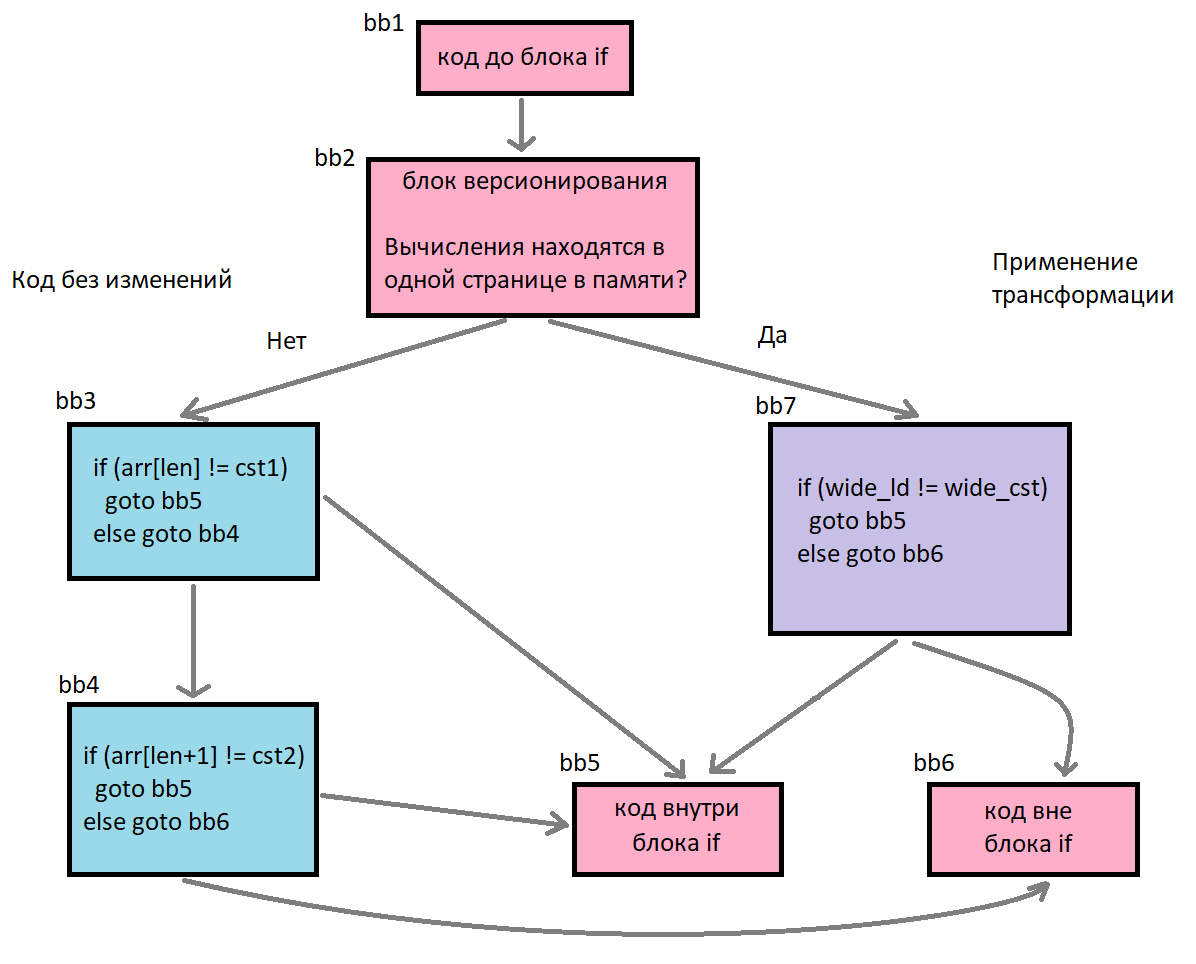
\includegraphics[scale=0.5]{versioning.png}
    \caption{Результат версионирования после применения оптимизации}
    \label{vers}
\end{figure}

Поскольку предложенный алгоритм предполагает динамическую проверку, что все векторизуемые элементы находятся в одной странице в памяти (подробнее в главе 4.1), необходимо использовать версионирование кода непосредственно перед потенциальным местом применения векторизации. Под версионированием в данном случае понимается следующее. В зависимости от результата проверки во время исполнения принимается решение о загрузке из памяти по отдельности, как это было изначально, или целиком одним обращением в память.

Проверка осуществляется следующим образом:

\begin{equation}
    addr\_last \ \& \ (page\_size - 1) \ge N_{elements} * size_{element} - 1,
\end{equation}

где 

\begin{itemize}
    \item $addr\_last$ - адрес крайнего элемента из векторизуемого набора
    \item $page\_size$ - размер страницы (по умолчанию 4096)
    \item $N_{elements}$ - количество элементов наборе
    \item $size_{element}$ - размер одного элемента
\end{itemize}

Таким образом, благодаря данной проверке можно убедиться, что все элементы массива, которые алгоритм собирается векторизовать лежат в одной странице в памяти. Чтобы использовать проверку во время исполнения необходимо создать новый базовый блок перед найденной цепочкой векторизуемых базовых блоков. Назовем этот базовый блок \textit{версионным}. Поскольку в зависимости от результата проверки принимается решение о том, чтобы применять трансформацию или нет, из него должно выходить две дуги, ведущие к соответственным местам в коде. Пример того, как работает версионирование представлен на рисунке ~\ref{vers}. Здесь под $wide\_ld$ понимается уже векторизованная загрузка элементов из памяти, а под $wide\_cst$ - объединение двух констант в одну тем же способом, представленным в главе 4.2.


За счет применения трансформации удается сократить количество косвенных переходов, поскольку вместо вычислений нескольких условий происходит вычисление лишь одного (рис. ~\ref{spec})

\begin{figure}[!htb]
    \centering
    \includesvg[scale=0.9]{speculate.svg}
    \caption{Результат версионирования после применения оптимизации}
    \label{spec}
\end{figure}

\subsection{Ограничения предлагаемого подхода}

Несмотря на преимущества, которые дает данная оптимизация, все же есть некоторые ограничения, которые накладывает данный подход. Большинство из них уже были упомянуты ранее.

\begin{enumerate}
    \item Отсутствие поддержки векторных инструкций
    \item Возможный регресс в определенных ситуациях
    \item Поддержка только операций чтения из памяти, отсутствие поддержки операций записи в память
\end{enumerate}

Предложенный алгоритм имеет возможность быть улучшенным и доработанным в будущем. Все вышесказанные ограничения могут быть решены, что оставляет поле для возможности дальнейшей работы, новых задач и результатов.
\newpage
